\section{Task Definition}
\label{sec:task}

Each document is parsed into an ordered tree of headings, sections, source chunks, and tables. Let $C$ denote the source chunks and $\mathcal{G}=(V,E,\tau_V,\tau_E)$ the typed evidence graph.

For a natural-language query $q$, the text task returns a ranking
\begin{equation}
R_C(q)=(c_1,c_2,\ldots), \qquad c_i\in C.
\end{equation}
Only source chunks confirmed by human reviewers, denoted $C_q^*$, count as relevant. A generated question, section summary, table summary, document node, or shortage entity cannot satisfy a text Gold judgment.

The structured task returns paths
\begin{equation}
P_G(q)=\{p_1,p_2,\ldots\}, \qquad p_i=(v_1,e_1,v_2,\ldots,v_k),
\end{equation}
with edge direction and source metadata preserved. A path succeeds when an accepted node and edge sequence appears in the first $K$ candidates. Structured nodes never enter text Hit@$K$, reciprocal rank, or nDCG.

The interface may display a passage and a path together, but their evidential roles remain explicit. \Cref{fig:dual-path} summarizes how an analyst request invokes text retrieval, structured relation-chain retrieval, or both while preserving this distinction.

\begin{figure}[!t]
  \centering
  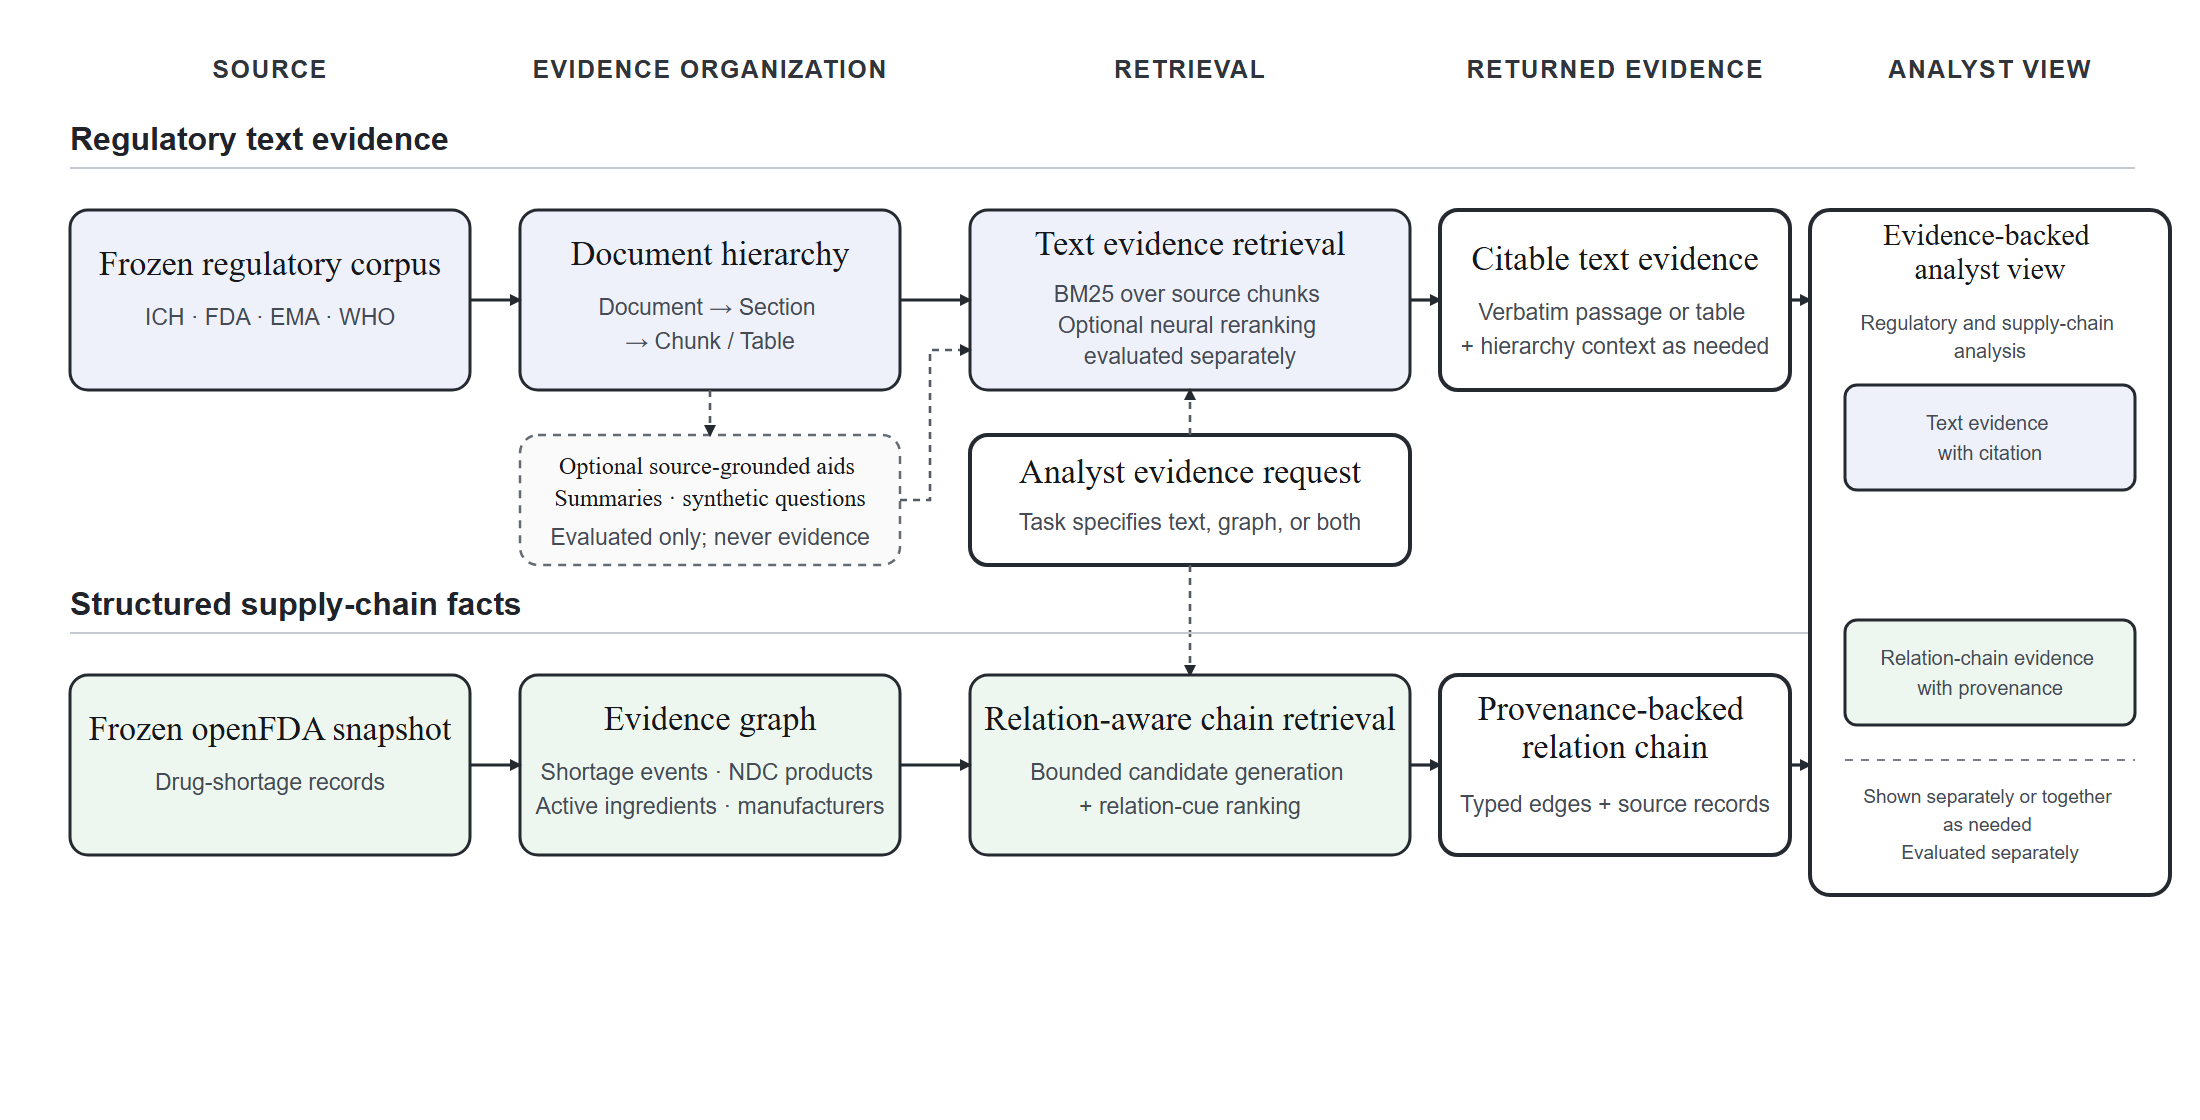
\includegraphics[width=\linewidth]{figures/dual_path_framework.png}
  \caption{Overview of the proposed dual-path auditable evidence retrieval framework. Analyst requests may invoke text retrieval, structured relation-chain retrieval, or both. Source-grounded summaries and synthetic questions were evaluated as optional retrieval aids but never treated as evidence; returned evidence remains a citable source passage, table, or provenance-bearing graph record.}
  \label{fig:dual-path}
\end{figure}
